\documentclass[bachelor, och, labwork]{shiza}

\usepackage[utf8]{inputenc}
\usepackage{graphicx}

\usepackage[sort,compress]{cite}
\usepackage{amsmath}
\usepackage{amssymb}
\usepackage{amsthm}
\usepackage{fancyvrb}
\usepackage{longtable}
\usepackage{array}
\usepackage[english,russian]{babel}
\usepackage{minted}

\usepackage{tempora}


% \usepackage[colorlinks=false]{hyperref}


\newcommand{\eqdef}{\stackrel {\rm def}{=}}


\begin{document}

\title{Алгоритмы алгебры и теории чисел}

\course{4}

\group{431}

\napravlenie{10.05.01 "--- Компьютерная безопасность}


\author{Никитина Арсения Владимировича}


\satitle{доцент}
\saname{А.\,С.\,Гераськин}


\date{2022}

\maketitle

% Включение нумерации рисунков, формул и таблиц по разделам
% (по умолчанию - нумерация сквозная)
% (допускается оба вида нумерации)
%\secNumbering


\tableofcontents

\section{Задание лабораторной работы}

Осуществить проверку чисел на простоту с помощью теста Рабина-Миллера

\section{Теоретическая часть}

\begin{center}
    \textit{Формулировка теста}
\end{center}

Пусть $n$ --- простое число и $n-1=2^{s}d$, где $d$ --- нечётно. Тогда 
$\forall a \in \mathbf{Z} _n$ ыполняется хотя бы одно из условий:

\begin{center}
    1. $a^{d}\equiv 1{\pmod {n}}$

    2. Существует целое число $r < s$ такое что $a^{2^{r}d}\equiv -1{\pmod {n}}$
\end{center}

\begin{center}
    \textit{Доказательство}
\end{center}

Если это утверждение (условие 1 или 2) выполняется для некоторых чисел 
$a$ и $n$ (не обязательно простого), то число $a$ называют \textit{свидетелем простоты} 
числа $n$ по Миллеру, а само число $n$ --- вероятно простым.

(При случайно выбранном $a$ вероятность ошибочно принять составное число за 
простое составляет 25\%, но её можно уменьшить, выполнив проверки для других $a$.

В случае когда выполняется контрапозиция доказанного утверждения, то есть 
если найдётся число $a$ такое, что:

\begin{center}
    $a^{d} \not\equiv 1\pmod{n}$ и $\forall r:\ 0\le r\le s-1:\ a^{2^rd} \not\equiv -1\pmod{n},$
\end{center}

то число $n$ не является простым. В этом случае число $a$ называют свидетелем того, 
что число $n$ составное.

Идея теста заключается в том, чтобы проверять для случайно выбранных 
чисел $a<n$, являются ли они свидетелями простоты числа $n$. Если найдётся 
свидетель того, что число составное, то число действительно является составным. 
Если было проверено $k$ чисел, и все они оказались свидетелями простоты, то число 
считается простым. Для такого алгоритма вероятность принять составное число за 
простое будет меньше $(1/4)^{k}$.


\section{Практическая часть}
\subsection{Пример работы алгоритма}
\begin{figure}[H]
    \centering
    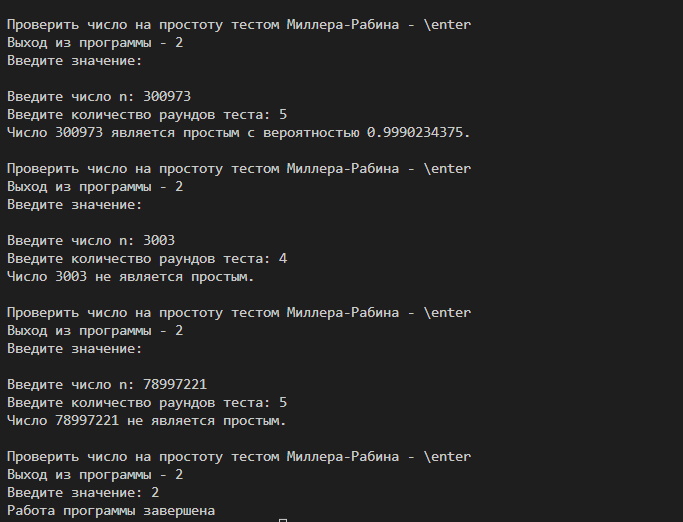
\includegraphics[width=0.8\textwidth]{pic1.png}
    \caption{}
\end{figure}

\setminted[python]{linenos,breaklines=true, fontsize=\small, style=bw}
    \subsection{Код программы, реализующей рассмотренный алгоритм}
        \inputminted{python}{lab7.py}

\end{document}